% Author: Matthew Turner

\documentclass[11pt,letterpaper]{article}
% \documentclass[11pt]{report}
% \documentclass{report}
% \documentclass{book}
\usepackage[bookmarks]{hyperref}
\usepackage{amssymb,amsmath}
% \usepackage{fullpage}
\usepackage{tabulary}
\usepackage{tabularx}

% \usepackage[margin=1.00in]{geometry}
\usepackage[margin=0.90in]{geometry}
\usepackage{float}

\usepackage[title]{appendix}

\usepackage{caption}
\usepackage{booktabs}
\usepackage{pslatex}
\usepackage{apacite}
\usepackage{subcaption}
\usepackage{pgfplots}
\usepackage{wrapfig}
\usepackage[english]{babel}
\usepackage{lmodern}
\usepackage{setspace}
\doublespace
% \usepackage{url}
\usepackage{bigfoot}
\usepackage[export]{adjustbox}
\setlength\intextsep{0pt}
\hypersetup{linktocpage}

\usepackage{graphicx}

\title{\vspace{-1in}Identity signaling model progress}

\author{} %{Matthew A.~Turner}}

\begin{document}
\maketitle
\tableofcontents

\section{Notes and planned improvements}

Notes:
\begin{itemize}
  \item All results are with 100 trials run to $t=T=500$ timesteps.
  \item On minority experiments:
    \begin{itemize}
      \item Restricted minority prevalence to be $\rho^{minor}\geq0.1$ in main plots, focusing
        on three exemplary cases. Full minority results, including $\rho^{minor}=0.05$,
        for many more values of homophily, $w$, are given in Appendix.
      \item I found through trial and error that difference between prevalence of 
        covert/churlish among minority and majority group at $t=T$ should be the
        relevant measure for the minority experiments. It matches with the
        heatmaps in this section, which I think tell a complementary story.
    \end{itemize}
\end{itemize}

Planned improvements:
\begin{itemize}
  \item Make all heatmap x and y axes match. All will have x-axis be 
    \emph{homophily} and all y-axes will be either \emph{disliking penalty},
    $d=\delta$, or \emph{relative covert receptivity}, $r/R$. 
    The best, model use of axes currently is in the invasion experiments.
  \item Combine four ``Basic'' heatmaps into one figure in matplotlib with 
    shared axes as explained above.
  \item Combine four ``Minority'' heatmaps into one figure in matplotlib with 
    shared axes as explained above.
  \item Improve data aggregation/reduction in covert-churlish correlation
    plots. Some sort of improved averaging should help readability. Get 
    closer to publication-ready annotations in correlation plots.
\end{itemize}

\section{Model}

Parameter table

\begin{table}[H]
  \centering
  \begin{tabular}{cp{6in}}
  \toprule
    Variable & Description \\
  \midrule
    $w$ & Homophily, which determines the level of assortment \\
    $d$ & Penalty for one individual disliking another in payoff \\
    $\delta$ & Additional penalty if both members of a dyad dislike one another \\
    $R$ & Receptivity of overt signaling---average fraction of population receive
      an overt signal. \\
    $r$ & Receptivity of covert signaling---average fraction of population receive
      a covert signal. \\
    $\rho_{i,t}$ & Prevalence of agents with signaling or receiving strategy $i$ at iteration/time step $t$. Add a superscript $minor$ or $major$ to indicate prevalence in 
    minority or majority subpopulations. \\
  \bottomrule
  \end{tabular}
\end{table}

\section{Results}

\subsection{Basic results starting from equilibrium}

\subsubsection{Density of covert signalers vs. $r/R$ and homophily, $w$}

Based on results from ``Evolution of covert signaling'' (``ECS''), I designed
the first agent-based model experiment to determine the dependence of the
density of covert signalers in the population ($\rho_C$) on
the receptiveness of the population to covert signals ($r$) and the
importance of homophily ($w$) to assortment. 

Here I set $R=0.5$, $s=0.25$, $d=\delta=0.25$,
and $N=100$. After signaling, agents go through 10 rounds of assortment/interaction,
followed by evolution after the 10 rounds of interaction. The model has been
run out to 100 timesteps where timeseries are nearly stable, though we will
want more timesteps for our final study, or perhaps adjust the number of 
assortment/interaction rounds up or down per timestep, to guarantee full 
stability.

I systematically varied $r/R$ by setting $R=0.5$ and varied 
$r \in \{0.0, 0.05, 0.1, \ldots, 0.45\}$ to get $r/R \in \{0.0, 0.1, \ldots, 0.9\}$.
I varied homophily identically to $r$, $w \in \{0.0, 0.5, \ldots, 0.45\}$. Note
that both $r$ and $w$ are bounded above by 0.5.

\begin{figure}[H]
  \centering
  \begin{subfigure}{0.49\textwidth}
    \centering
    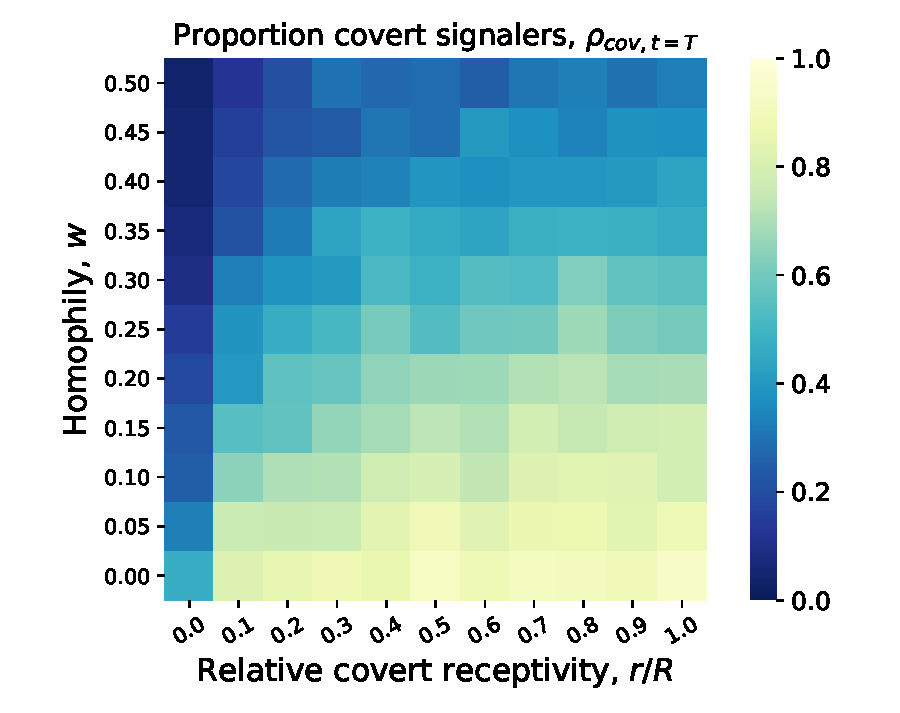
\includegraphics[width=\textwidth]{Figures/basic_receptivity_signaling.pdf}
    \caption{Density of covert signalers.}
  \end{subfigure}
  \begin{subfigure}{0.49\textwidth}
    \centering
    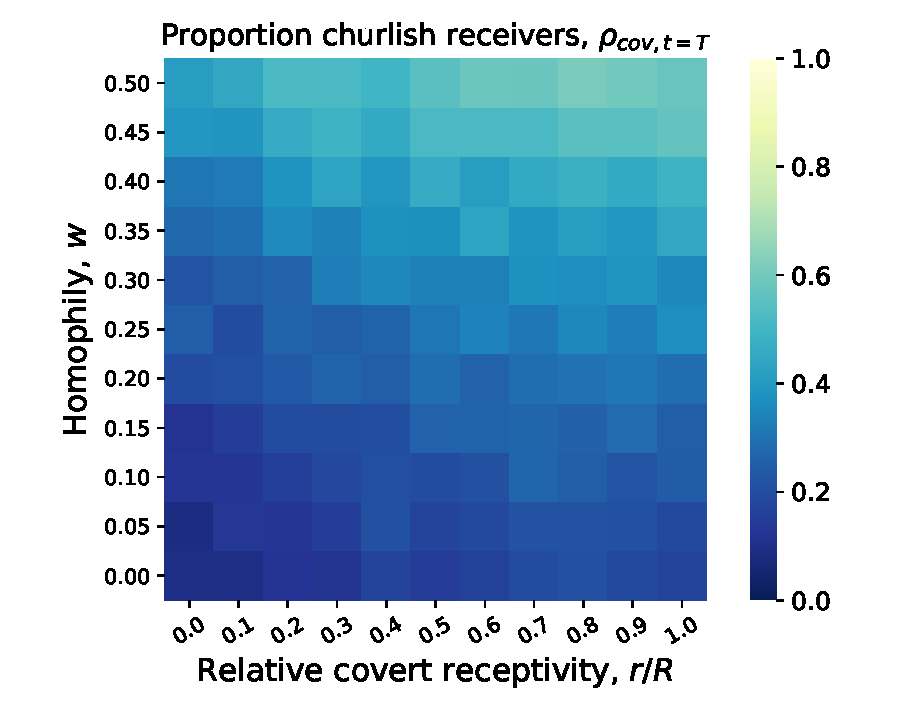
\includegraphics[width=\textwidth]{Figures/basic_receptivity_receiving.pdf}
    \caption{Density of churlish receivers.}
  \end{subfigure}
  
  \caption{Density of covert signalers and churlish receivers at $t=200$, 
    final timestep recorded in this preliminary experiment. Receptivity of
    overt signals is $R=0.5$.}
  \label{fig:dislikingHomophilyHeatmap}
\end{figure}


\subsubsection{Density of covert signalers vs. disliking penalty $d=\delta$ and homophily, $w$}

Here I co-vary the disliking penalties, which I set equal ($d=\delta$), and
homophily, $w$. Here, $r=0.25$ and $R=0.5$. 

Specifically, I vary $d=\delta \in \{0.0, 0.05, 0.1, \ldots, 0.45\}$
As in the above experiment, I set $w \in \{0.0, 0.5, \ldots, 0.45\}$.

\begin{figure}[H]
  \centering
  \begin{subfigure}{0.49\textwidth}
    \centering
    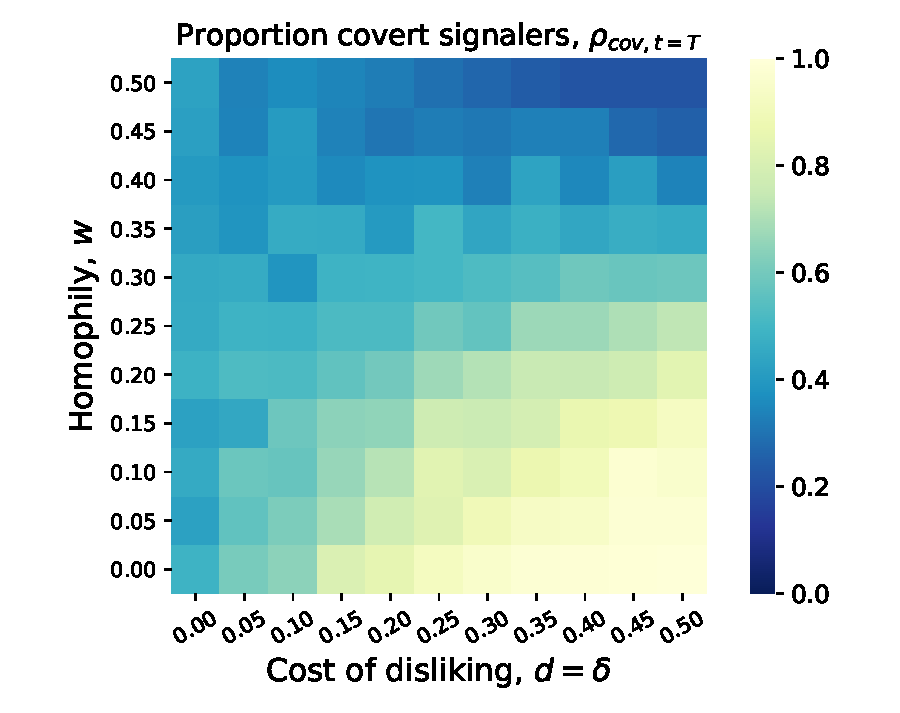
\includegraphics[width=\textwidth]{Figures/basic_disliking_signaling.pdf}
    \caption{Density of covert signalers.}
  \end{subfigure}
  \begin{subfigure}{0.49\textwidth}
    \centering
    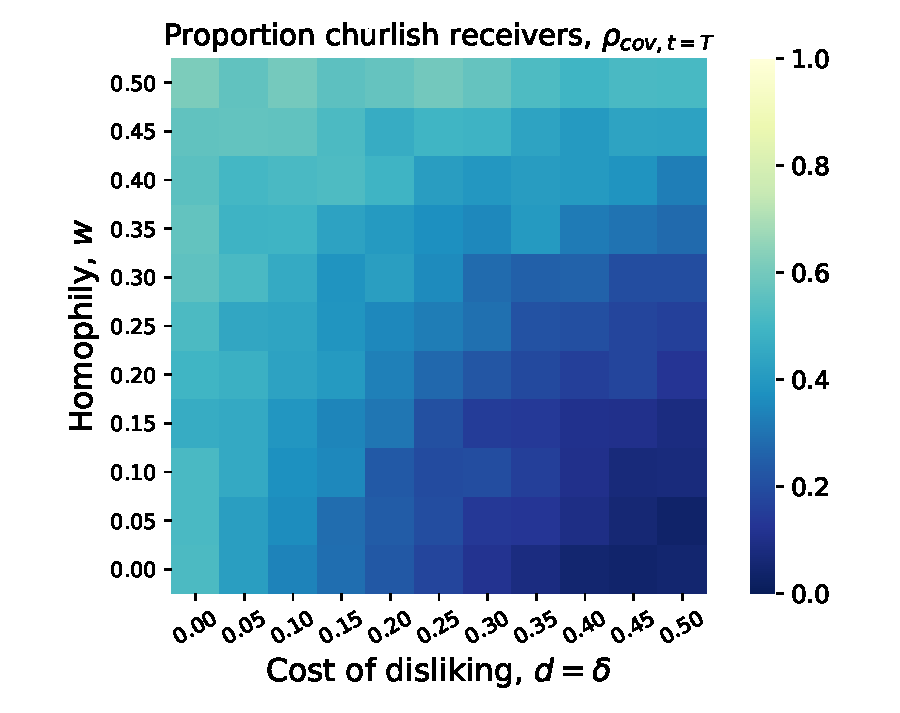
\includegraphics[width=\textwidth]{Figures/basic_disliking_receiving.pdf}
    \caption{Density of churlish receivers.}
  \end{subfigure}
  
  \caption{Density of covert signalers and churlish receivers at $t=200$, 
    final timestep recorded in this preliminary experiment. NEED TO MAKE THESE
    SQUARE AND UPDATE THEM WITH LATEST DATA RUN TO 100 TIMESTEPS.}
  \label{fig:dislikingHomophilyHeatmap}
\end{figure}


\subsubsection{Correlations between proportion of covert signalers and of churlish receivers}

\begin{figure}[H]
  \centering
  \begin{subfigure}{0.49\textwidth}
    \centering
    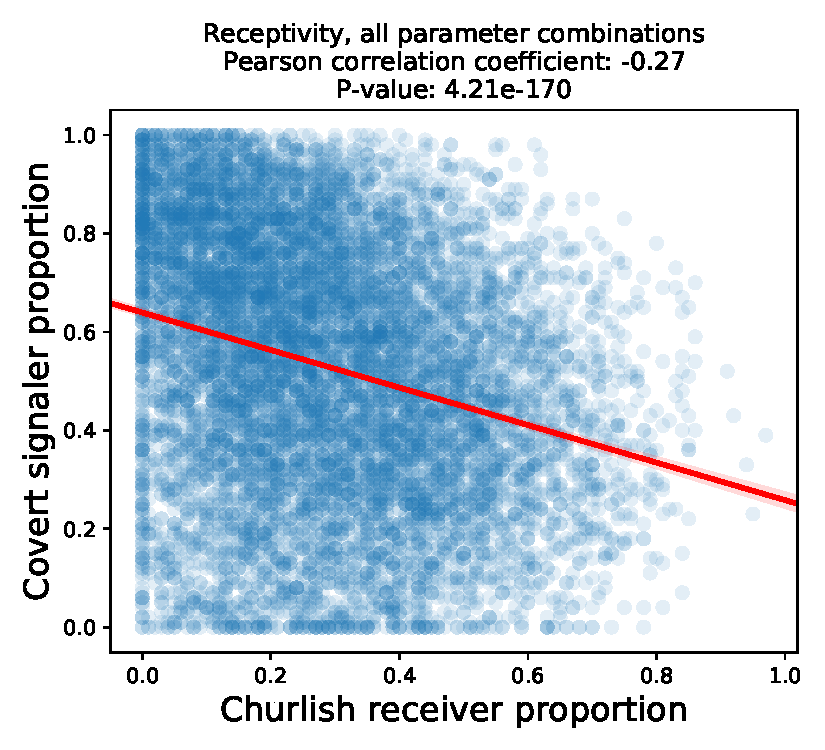
\includegraphics[width=\textwidth]{Figures/receptivity_allcombos_reg.pdf}
    \caption{}
    \label{fig:}
  \end{subfigure}
  \begin{subfigure}{0.49\textwidth}
    \centering
    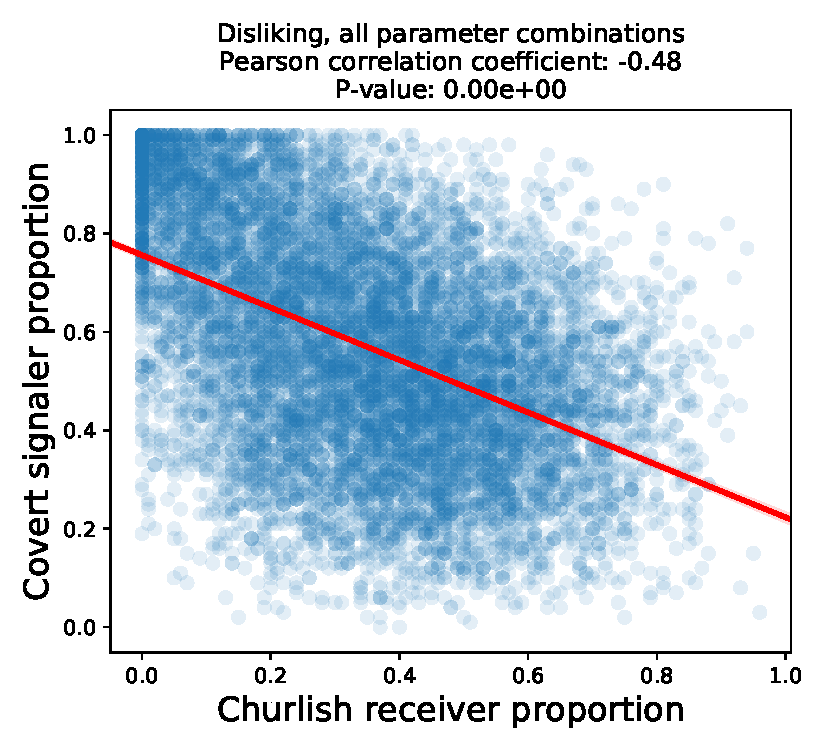
\includegraphics[width=\textwidth]{Figures/disliking_allcombos_reg.pdf}
    \caption{}
    \label{fig:}
  \end{subfigure}
  \caption{Correlation between proportion of covert signalers and proportion of
    churlish receivers for all tested parameter combinations in both 
    receptivity (a) and disliking (b) experiments. (NEED TO CHECK HOW I'M AVERAGING
    HERE AND POSSIBLY AGGREGATE FURTHER AS A SMOOTHING FILTER.)}
  \label{fig:regressions}
\end{figure}

\subsection{Invasion}

In this experiment we begin with initial proportions, $\rho$ of one of the strategies
at 0.05 and consider this the ``invading'' strategy. $\rho_{cov,0}$ represents
the initial covert proportion, $\rho_{ov,0}$ the initial overt proportion,
$\rho_{ch,0}$ the initial churlish proportion, and $\rho_{gen,0}$ the 
initial generous proportion. We measure how often
a non-zero proportion of agents with the invading strategy manage to 
establish a permanent population, which we call invasion success. We calculated
invasion success for a number of experimental parameter settings, covarying
over disliking penalty ($d=\delta$) and homophily ($w$) in the first case,
and over relative covert receptivity ($r/R$) and homophily ($w$) 
in the second case (Figures~\ref{fig:cov-ov-invade} and~\ref{fig:ch-gen-invade}).

\begin{figure}[H]
  \centering
    \begin{subfigure}{0.49\textwidth}
      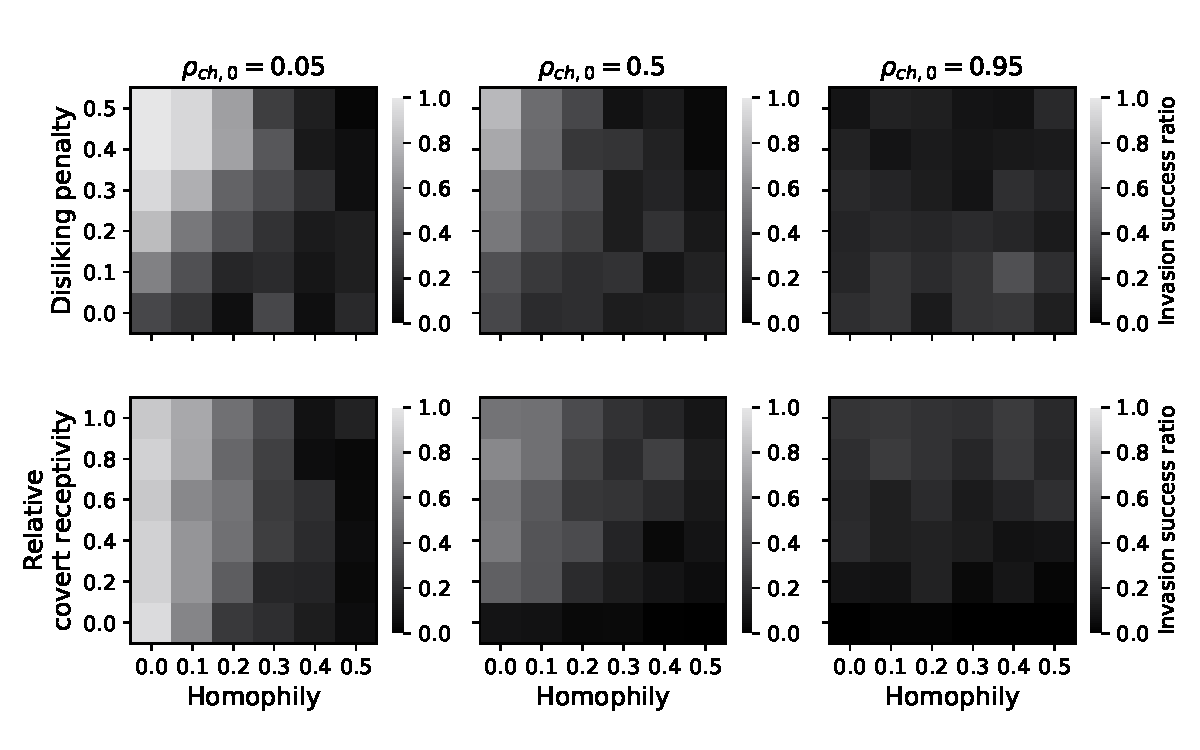
\includegraphics[width=\textwidth]{Figures/covert_invades.pdf}
      \caption{Covert invades, $\rho_{cov,0}=0.05$}
    \end{subfigure}
    \begin{subfigure}{0.49\textwidth}
      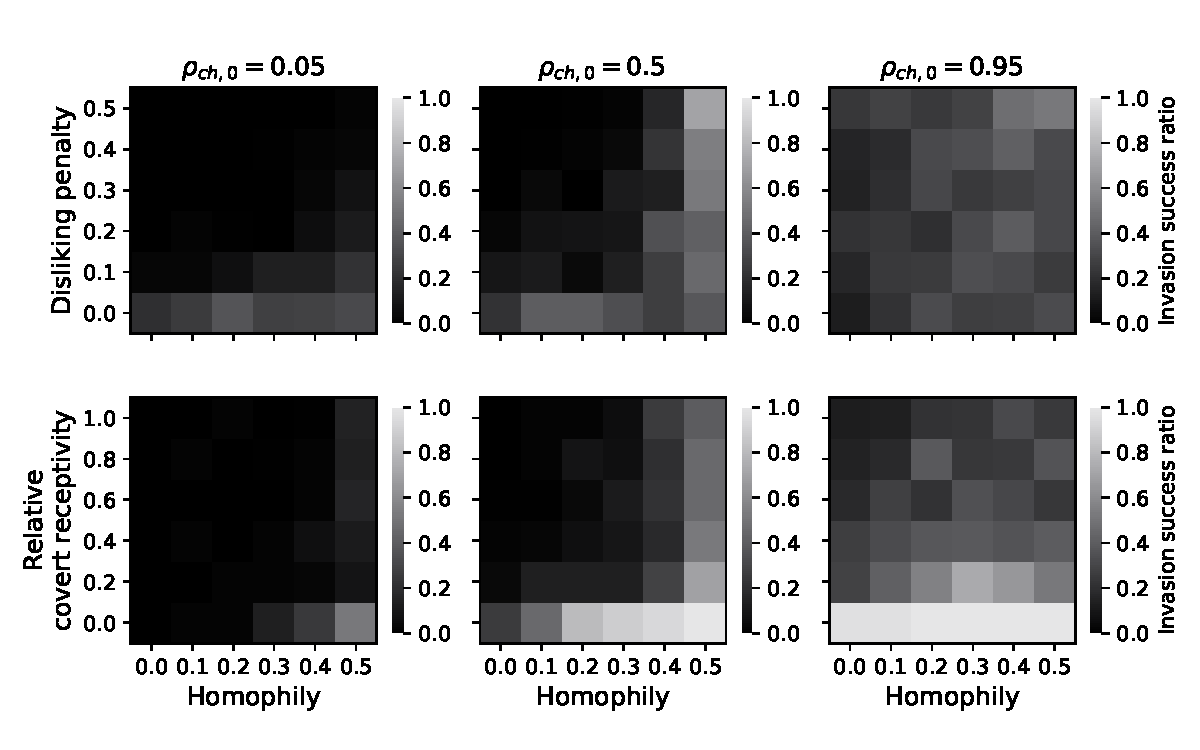
\includegraphics[width=\textwidth]{Figures/overt_invades.pdf}
      \caption{Overt invades, $\rho_{cov,0}=0.95$}
    \end{subfigure}
  \caption{Covert and overt sending strategy invasion success rates. 
    Lower homophily is more favorable for successful covert signaling invasion.
    This is due to lower homophily meaning agents cannot assort well into
    similar pairs prior to interaction.
    Similarly, greater homophily is more favorable for successful overt
    signaling invasion, where agents can better assort if they know each other's
    true traits. Unexpectedly, as covert receptivity increases, overt signaling
    is is more successful at invading and covert signaling is less successful
    at invading when the initial churlishness is high. When initial
    churlishness is small to moderate, the pattern is reversed.
  }
  \label{fig:cov-ov-invade}
\end{figure}

\begin{figure}[H]
  \centering
    \begin{subfigure}{0.49\textwidth}
      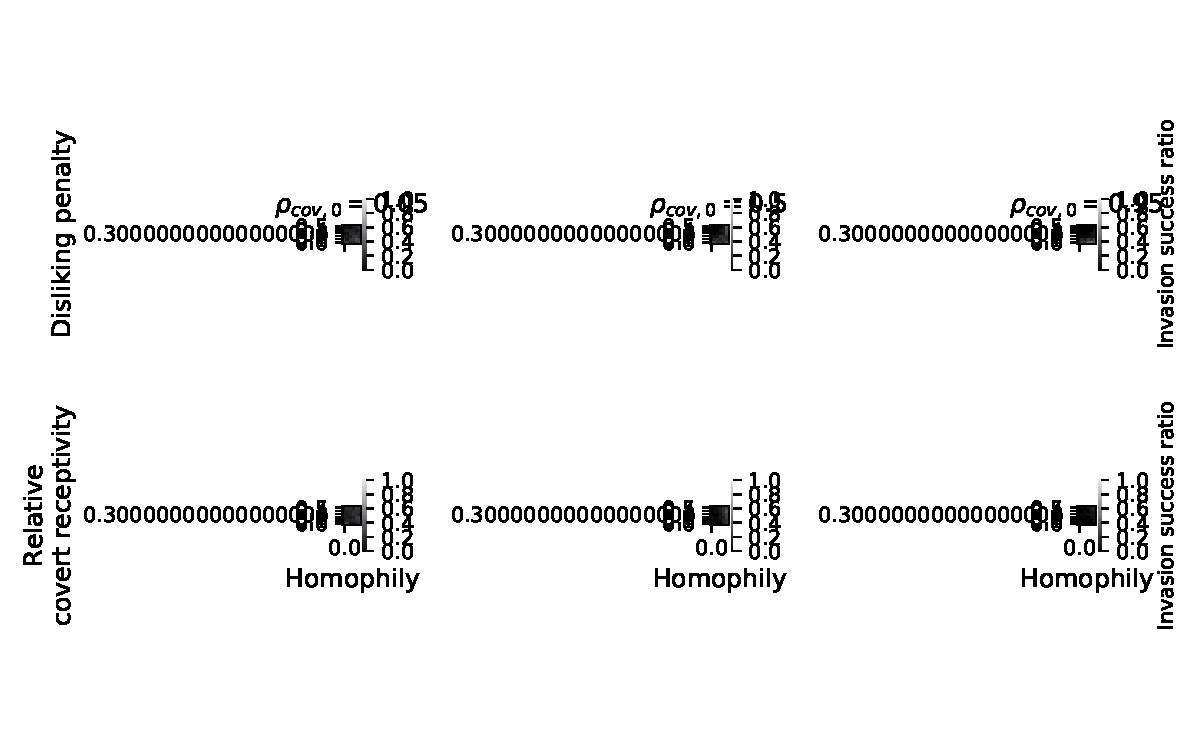
\includegraphics[width=\textwidth]{Figures/churlish_invades.pdf}
      \caption{Churlish invades, $\rho_{ch,0}=0.05$}
    \end{subfigure}
    \begin{subfigure}{0.49\textwidth}
      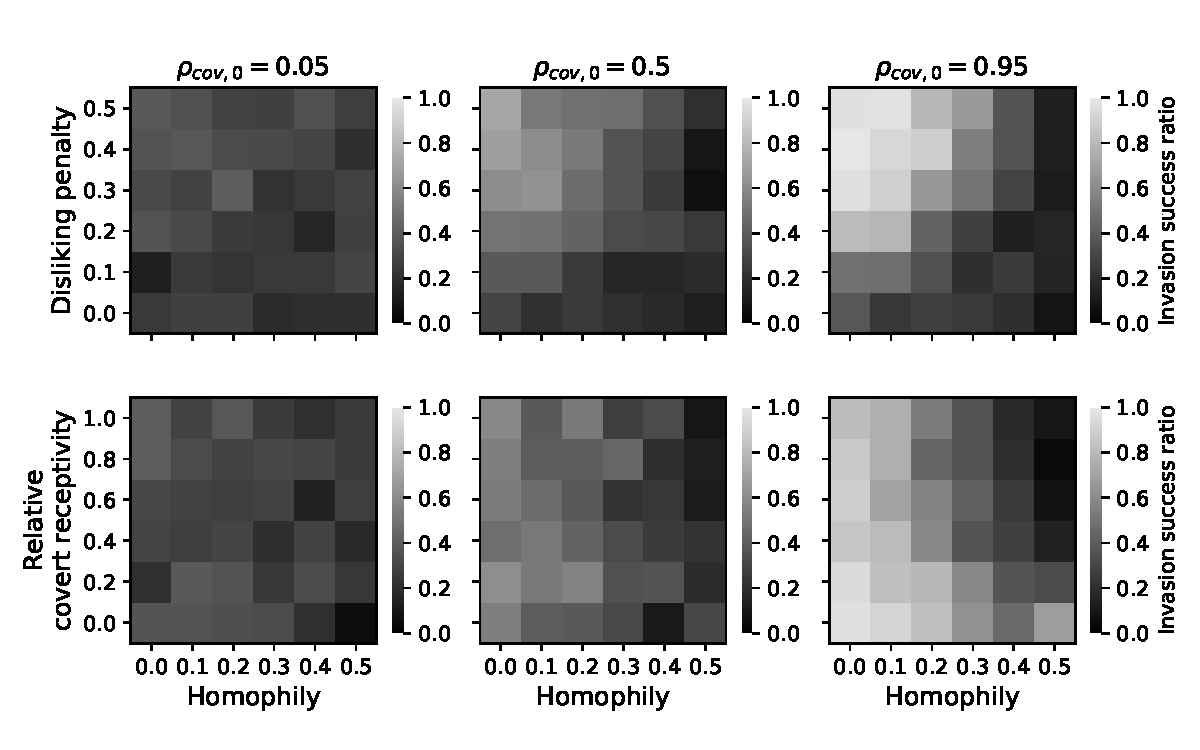
\includegraphics[width=\textwidth]{Figures/generous_invades.pdf}
      \caption{Generous invades, $\rho_{ch,0}=0.95$}
    \end{subfigure}
  \caption{Churlish and generous receiving strategy invasion success rates.
    For low to moderate rates of initial covert signaling there is not much
    of a pattern to invasion success. High values of homophily do seem to lead
    to more successful churlish invasion for moderate values of initial
    covert signalers. For large initial proportions of covert
    signalers, lower homophily favors generous invasion, which is more pronounced
    for larger disliking penalties.
  }
  \label{fig:ch-gen-invade}
\end{figure}


\subsection{Minority populations}

\begin{figure}[H]
  \centering
  \begin{subfigure}{0.31\textwidth}
    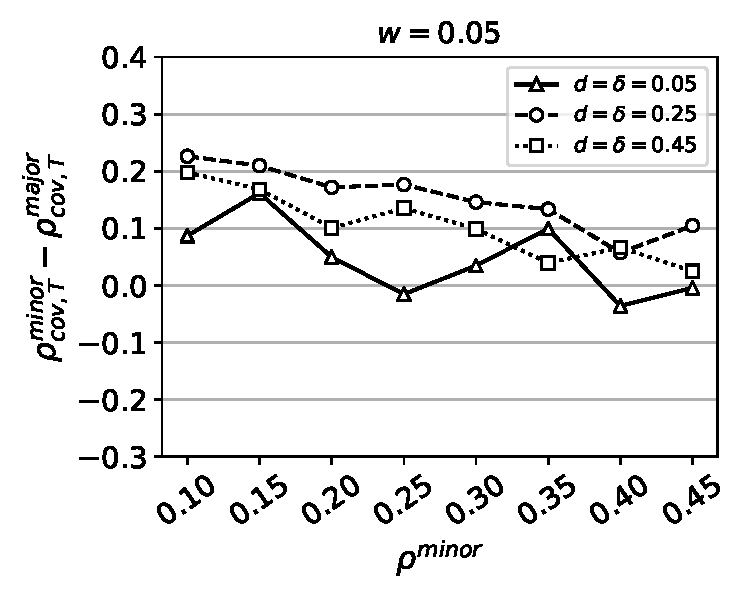
\includegraphics[width=\textwidth]{Figures/minority-homophily=0p05.pdf}
    \caption{}
  \end{subfigure}
  \begin{subfigure}{0.31\textwidth}
    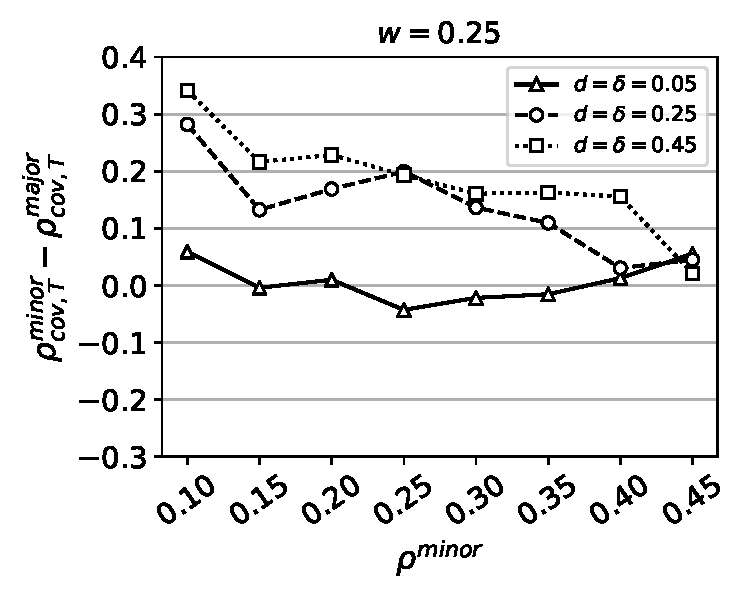
\includegraphics[width=\textwidth]{Figures/minority-homophily=0p25.pdf}
    \caption{}
  \end{subfigure}
  \begin{subfigure}{0.31\textwidth}
    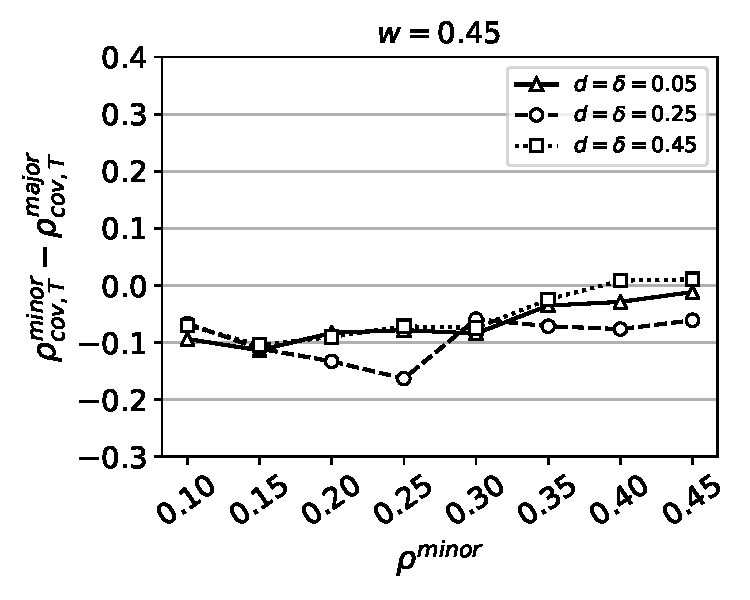
\includegraphics[width=\textwidth]{Figures/minority-homophily=0p45.pdf}
    \caption{}
  \end{subfigure}
  \caption{}
\end{figure}

\begin{figure}[H]
  \centering
  \begin{subfigure}{0.4\textwidth}
    \centering
    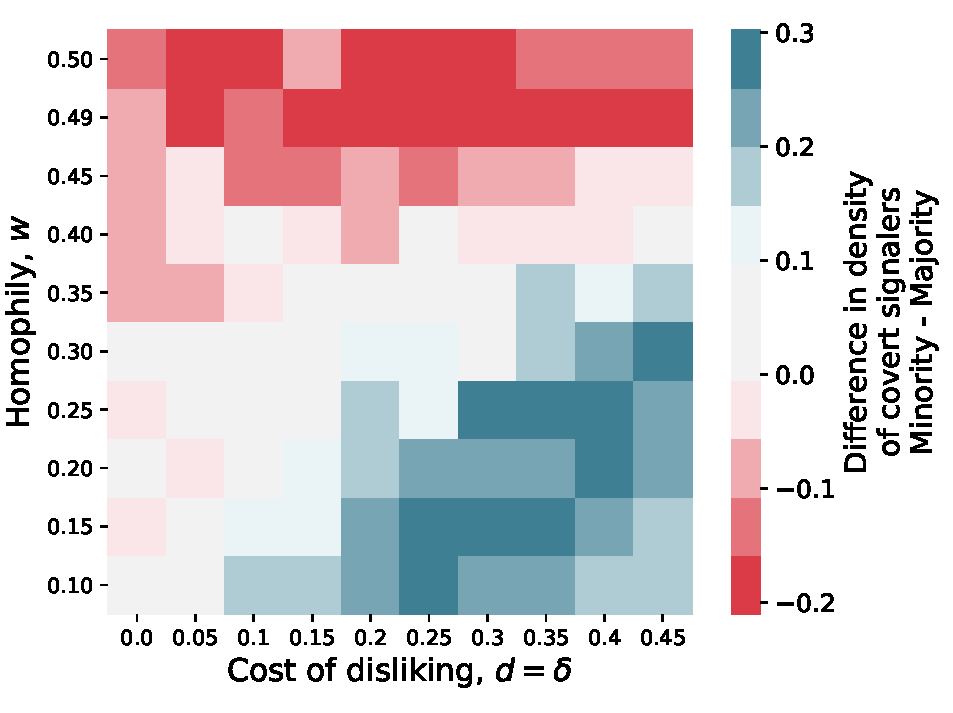
\includegraphics[width=\textwidth]{Figures/covert_signalers_diff_010.pdf}
    \caption{Prevalence of minority covert receivers; $\rho^{minor} = 0.10$.}
  \end{subfigure}
  \hfill
  \begin{subfigure}{0.4\textwidth}
    \centering
    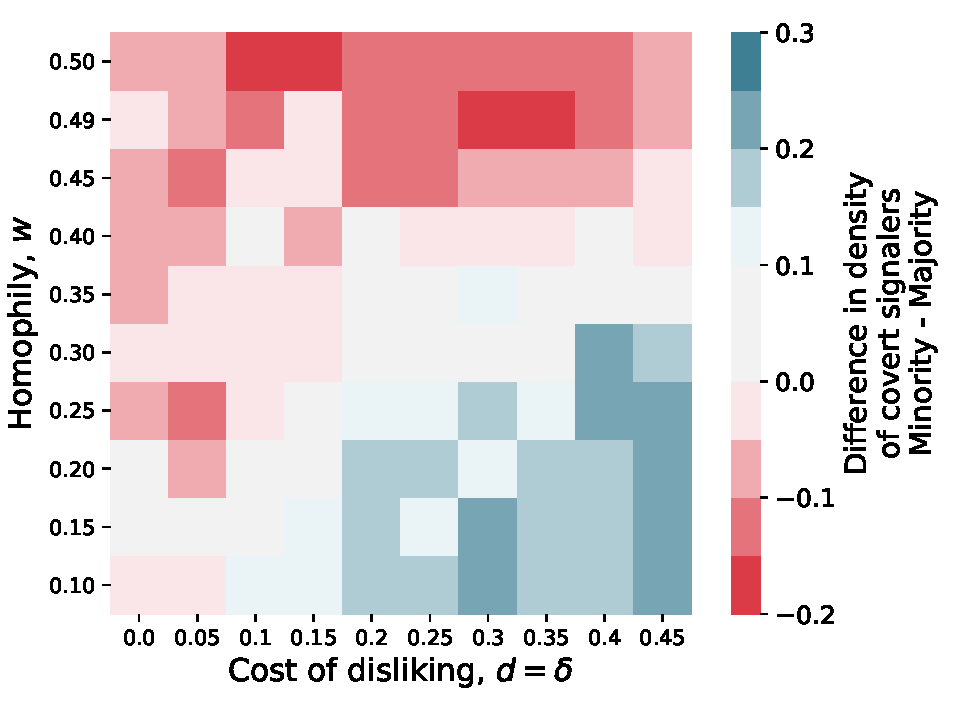
\includegraphics[width=\textwidth]{Figures/covert_signalers_diff_025.pdf}
    \caption{Prevalence of minority covert receivers; $\rho^{minor} = 0.25$.}
  \end{subfigure} \\[.25in]
  \begin{subfigure}{0.4\textwidth}
    \centering
    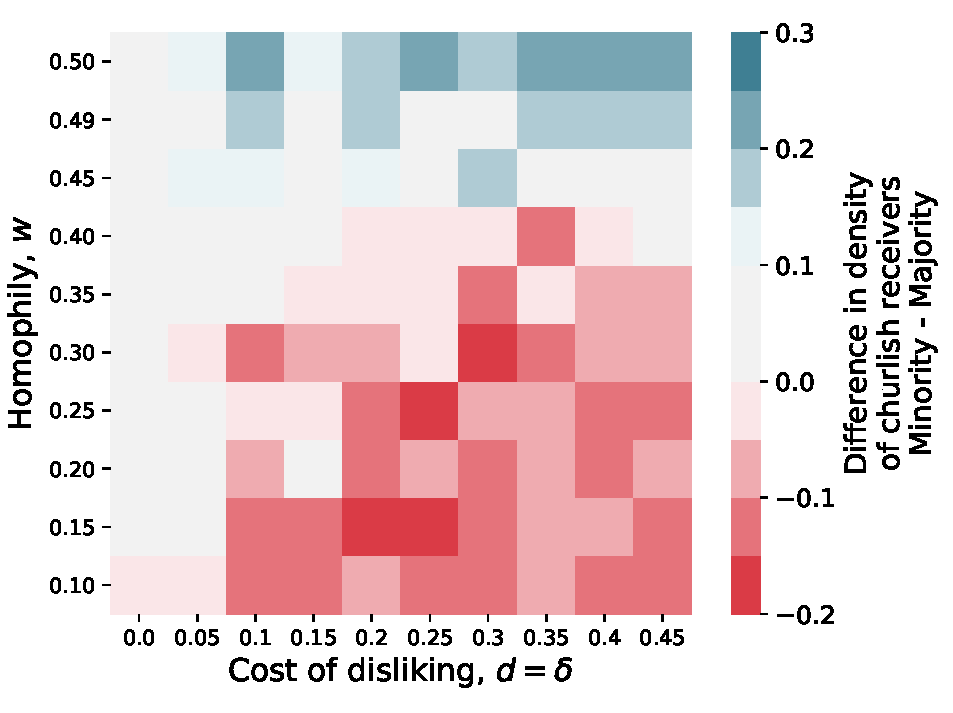
\includegraphics[width=\textwidth]{Figures/churlish_receivers_diff_010.pdf}
    \caption{Prevalence of minority churilsh receivers; $\rho^{minor} = 0.10$.}
  \end{subfigure}
  \hfill
  \begin{subfigure}{0.4\textwidth}
    \centering
    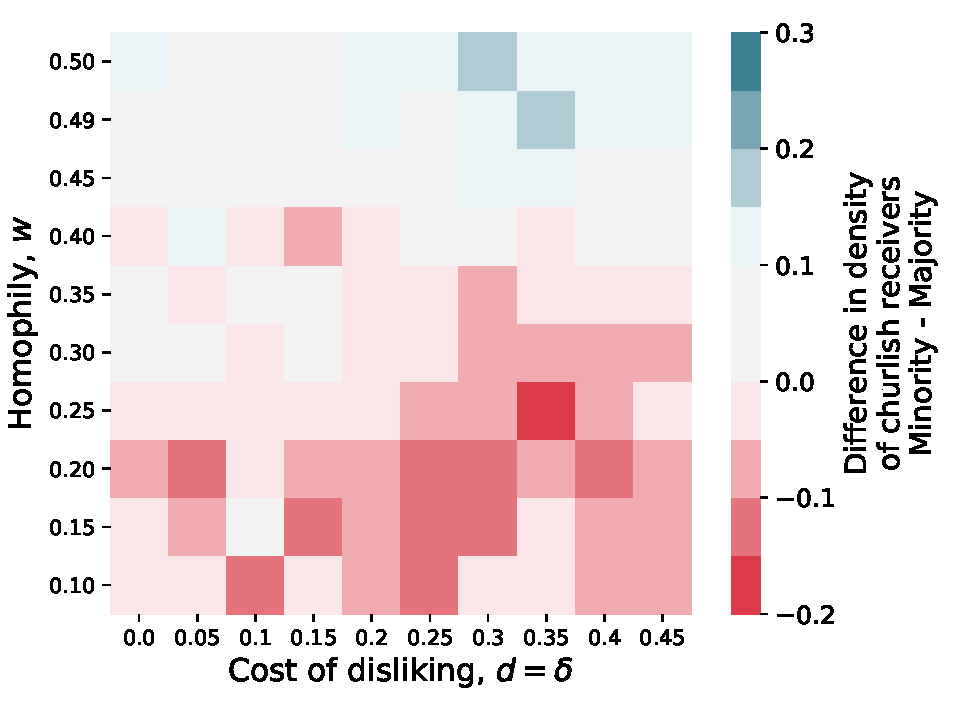
\includegraphics[width=\textwidth]{Figures/churlish_receivers_diff_025.pdf}
    \caption{Prevalence of minority churilsh receivers; $\rho^{minor} = 0.25$.}
  \end{subfigure}
  \caption{}
\end{figure}


\begin{appendices}

\section{Evolution in signaling and receiving strategies}

\begin{figure}[H]
  \centering
  \begin{subfigure}{0.49\textwidth}
    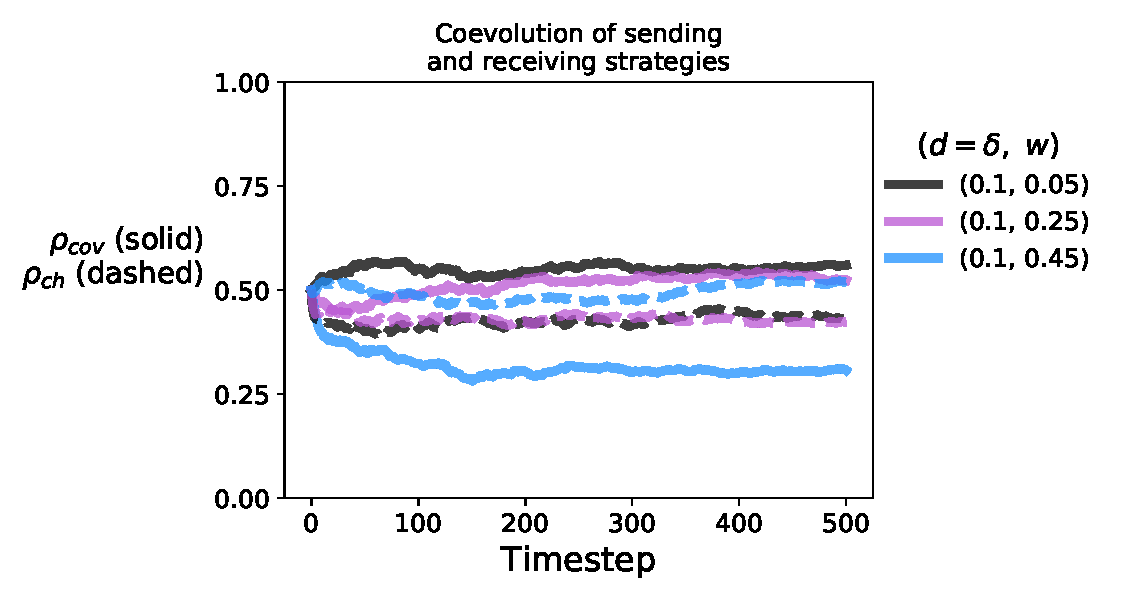
\includegraphics[width=\textwidth]{Figures/disliking_evo_d=0p1.pdf}
  \caption{}
  \end{subfigure}
  \begin{subfigure}{0.49\textwidth}
    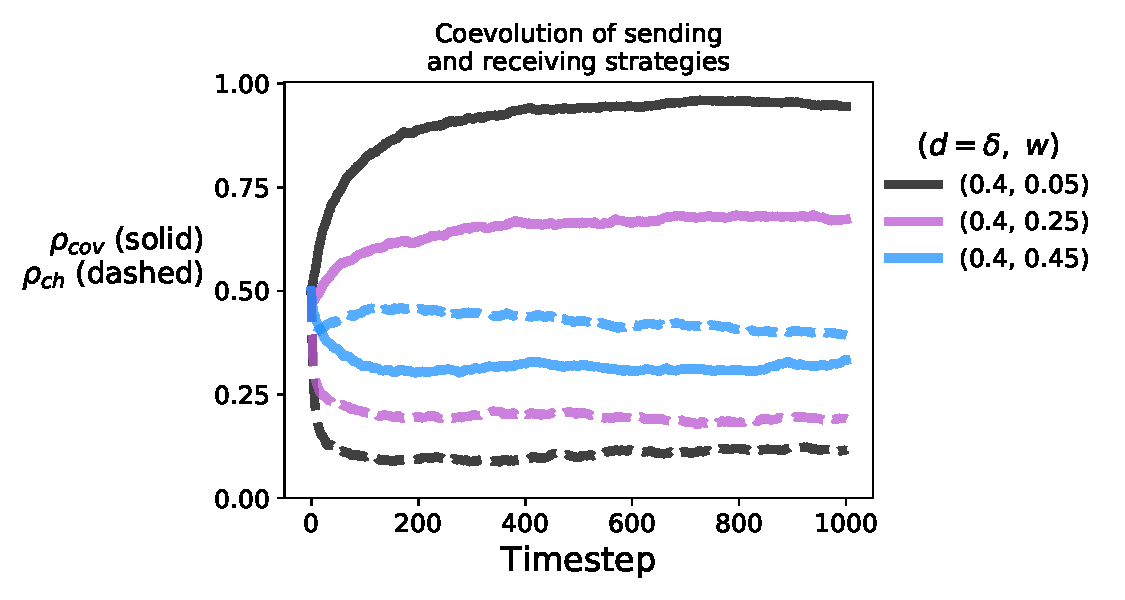
\includegraphics[width=\textwidth]{Figures/disliking_evo_d=0p4.pdf}
  \caption{}
  \end{subfigure} \\
  \begin{subfigure}{0.49\textwidth}
    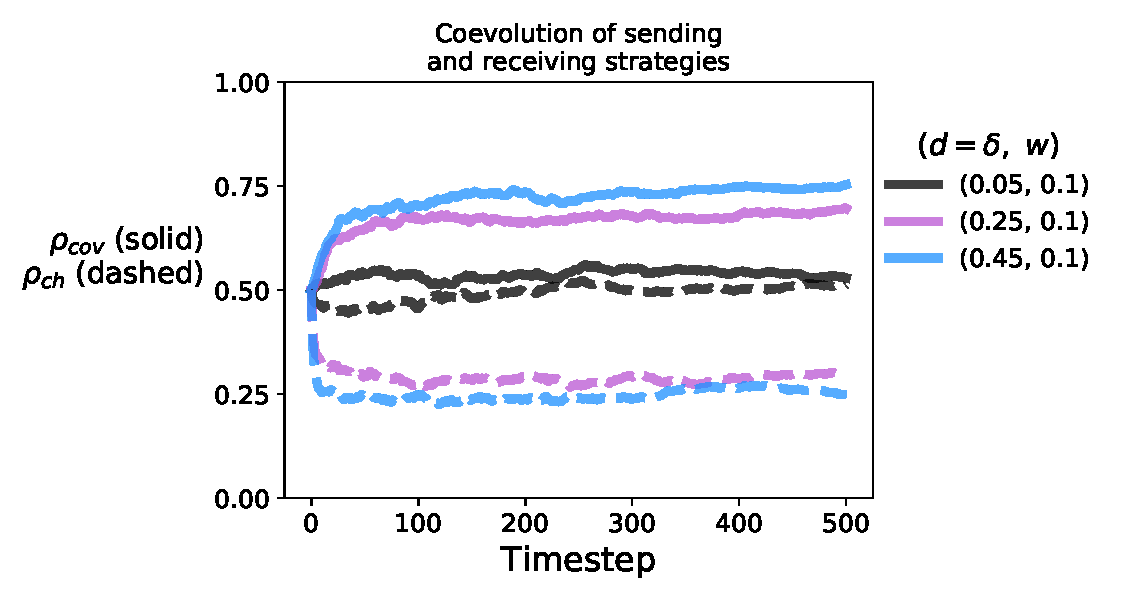
\includegraphics[width=\textwidth]{Figures/disliking_evo_w=0p1.pdf}
  \caption{}
  \end{subfigure}
  \begin{subfigure}{0.49\textwidth}
    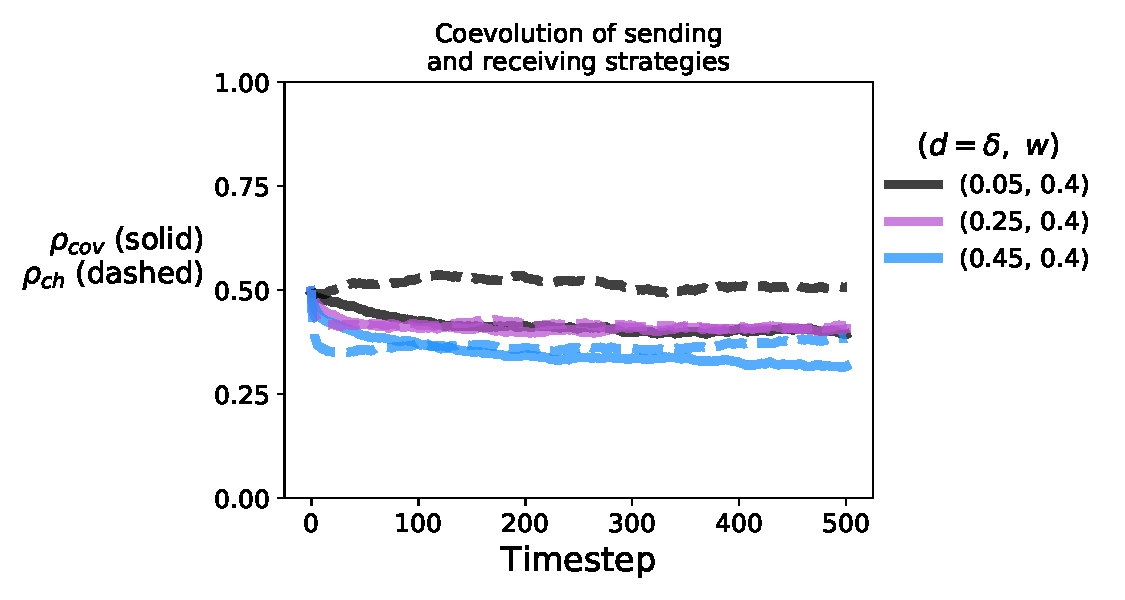
\includegraphics[width=\textwidth]{Figures/disliking_evo_w=0p4.pdf}
  \caption{}
  \end{subfigure}
  \caption{}
  \label{fig:}
\end{figure}

\begin{figure}[H]
  \centering
  \begin{subfigure}{0.49\textwidth}
    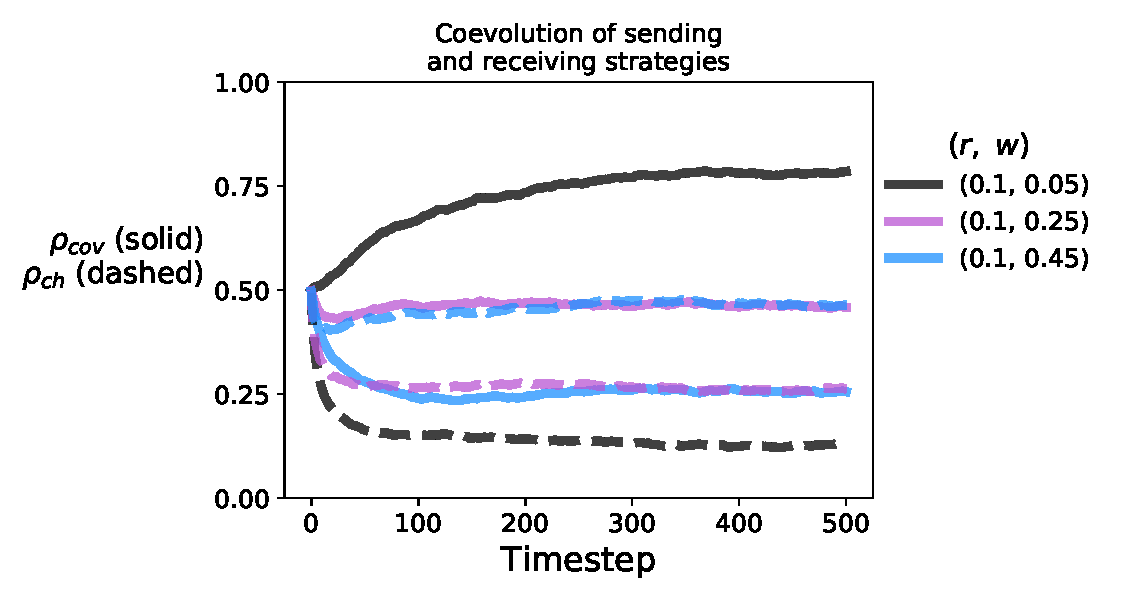
\includegraphics[width=\textwidth]{Figures/receptivity_evo_r=0p1.pdf}
  \caption{}
  \end{subfigure}
  \begin{subfigure}{0.49\textwidth}
    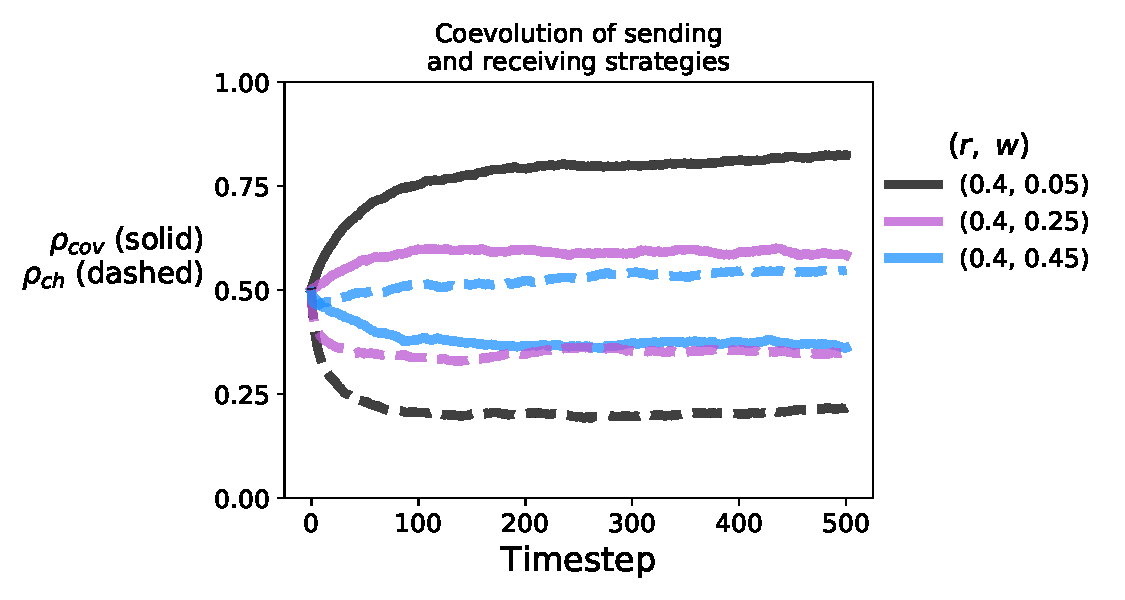
\includegraphics[width=\textwidth]{Figures/receptivity_evo_r=0p4.pdf}
  \caption{}
  \end{subfigure} \\
  \begin{subfigure}{0.49\textwidth}
    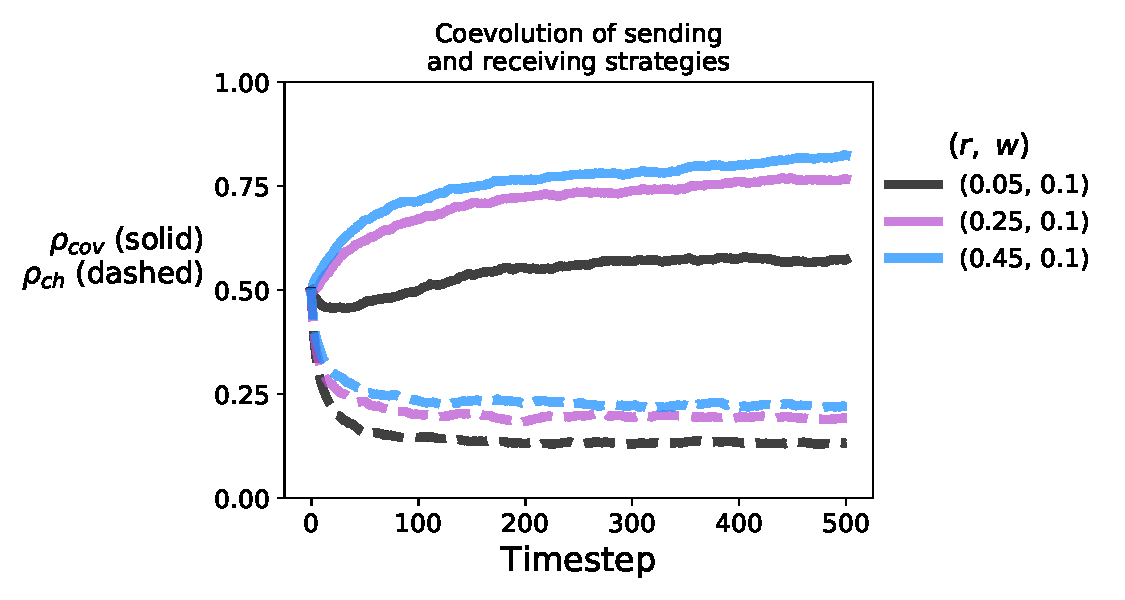
\includegraphics[width=\textwidth]{Figures/receptivity_evo_w=0p1.pdf}
  \caption{}
  \end{subfigure}
  \begin{subfigure}{0.49\textwidth}
    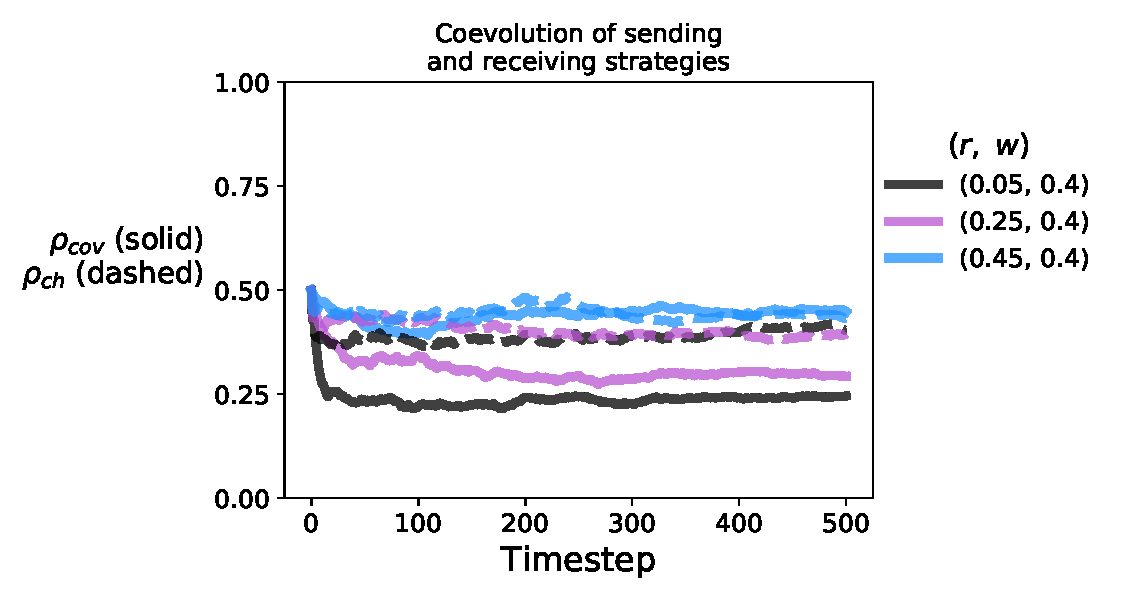
\includegraphics[width=\textwidth]{Figures/receptivity_evo_w=0p4.pdf}
  \caption{}
  \end{subfigure}
  \caption{}
  \label{fig:}
\end{figure}

\section{Complete minority experiment data}

Due to finite-size simulation extinction in small populations, from 0.05 to
0.1 we saw an increase in the relative prevalence of covert signaling among
minority individuals. 


\begin{figure}[H]
  \centering
  \begin{subfigure}{0.315\textwidth}
    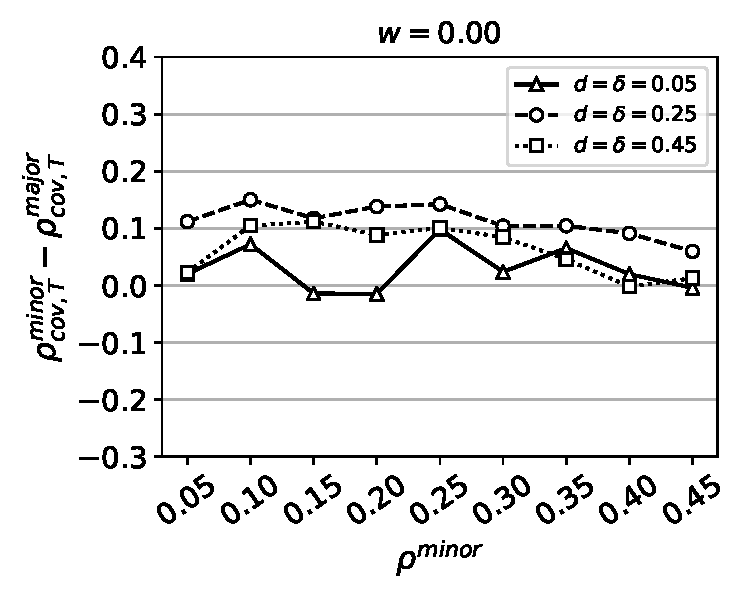
\includegraphics[width=\textwidth]{Figures/full-minority-homophily=0p00.pdf}
  \end{subfigure}
  \begin{subfigure}{0.315\textwidth}
    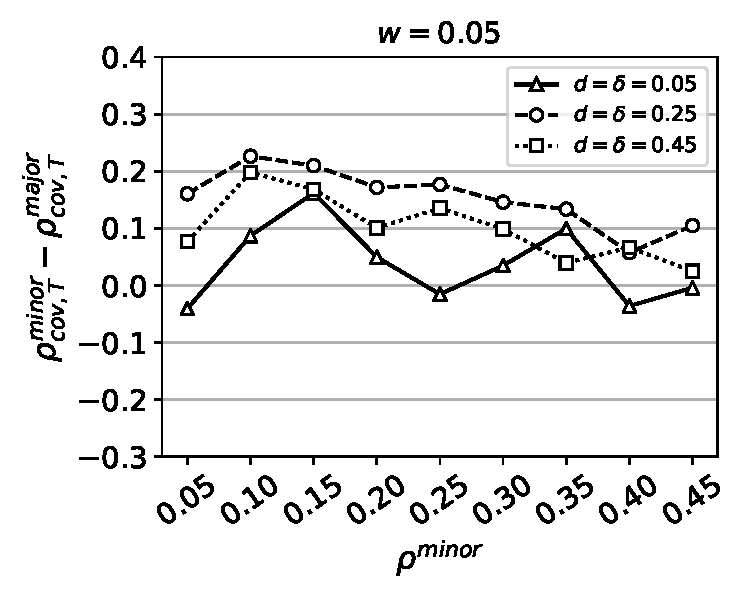
\includegraphics[width=\textwidth]{Figures/full-minority-homophily=0p05.pdf}
  \end{subfigure}
  \begin{subfigure}{0.315\textwidth}
    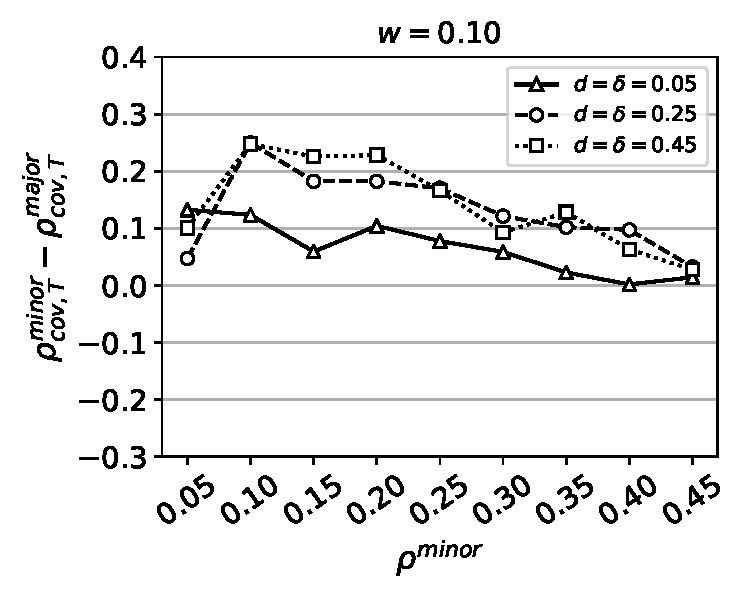
\includegraphics[width=\textwidth]{Figures/full-minority-homophily=0p10.pdf}
  \end{subfigure} \\
  \begin{subfigure}{0.315\textwidth}
    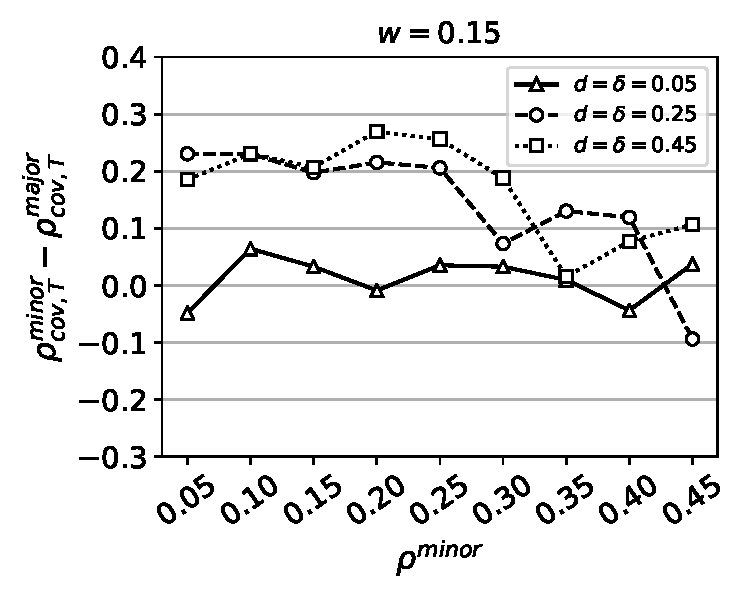
\includegraphics[width=\textwidth]{Figures/full-minority-homophily=0p15.pdf}
  \end{subfigure}
  \begin{subfigure}{0.315\textwidth}
    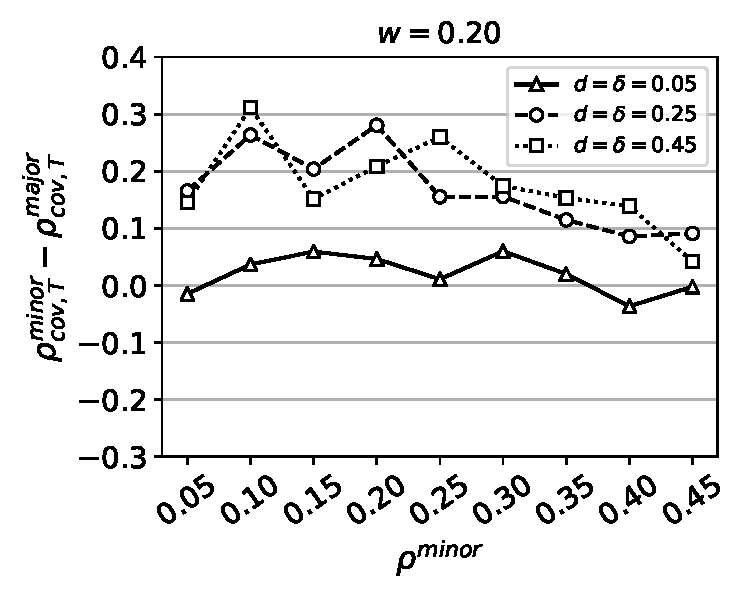
\includegraphics[width=\textwidth]{Figures/full-minority-homophily=0p20.pdf}
  \end{subfigure}
  \begin{subfigure}{0.315\textwidth}
    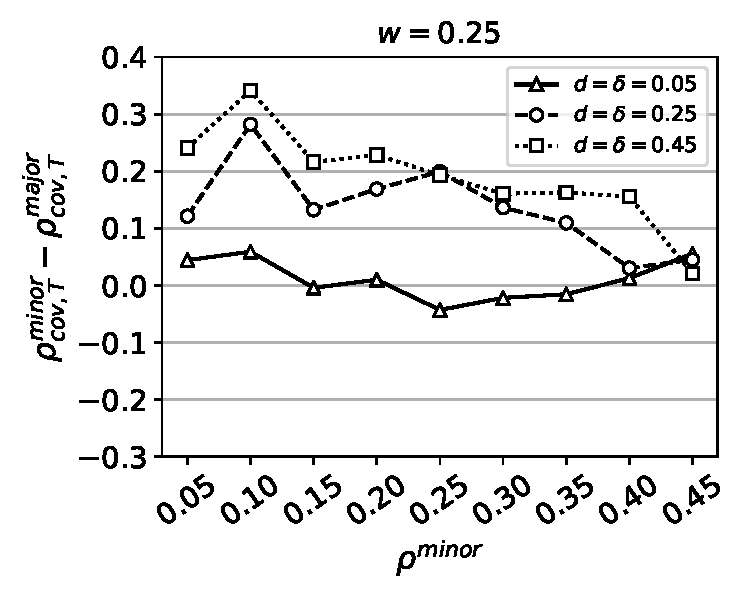
\includegraphics[width=\textwidth]{Figures/full-minority-homophily=0p25.pdf}
  \end{subfigure}
  \\
  \begin{subfigure}{0.315\textwidth}
    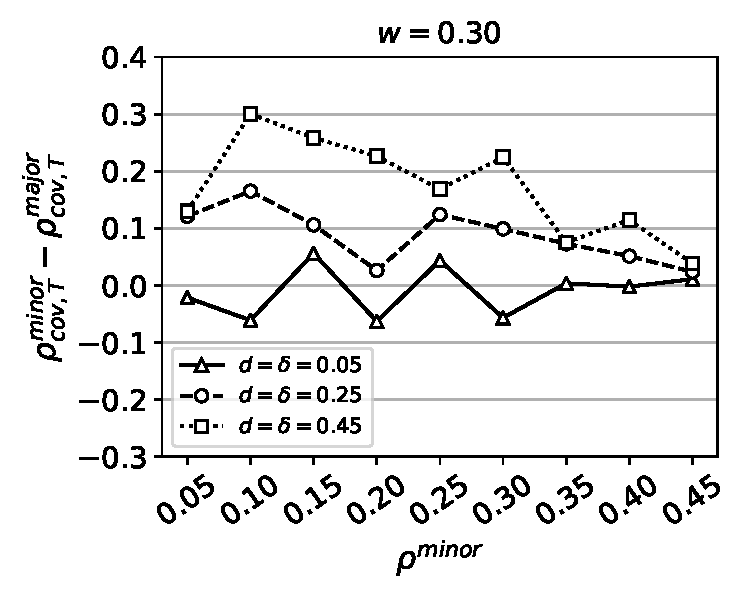
\includegraphics[width=\textwidth]{Figures/full-minority-homophily=0p30.pdf}
  \end{subfigure}
  \begin{subfigure}{0.315\textwidth}
    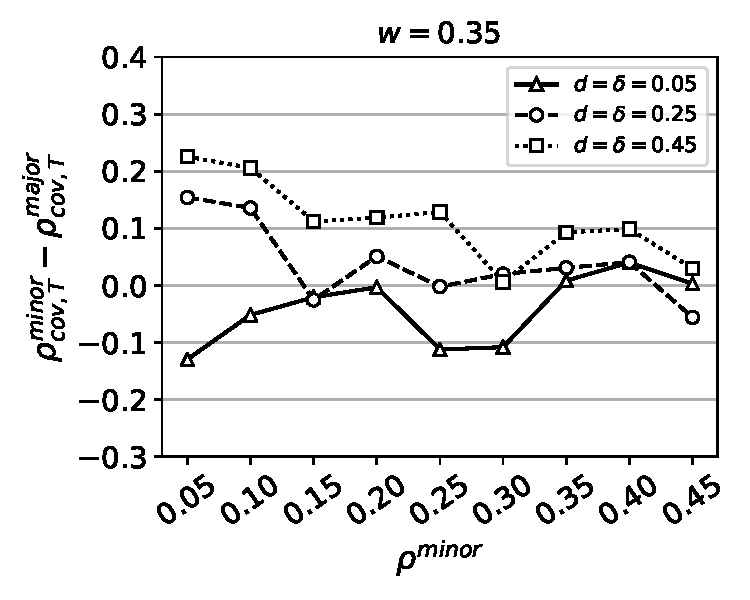
\includegraphics[width=\textwidth]{Figures/full-minority-homophily=0p35.pdf}
  \end{subfigure}
  \begin{subfigure}{0.315\textwidth}
    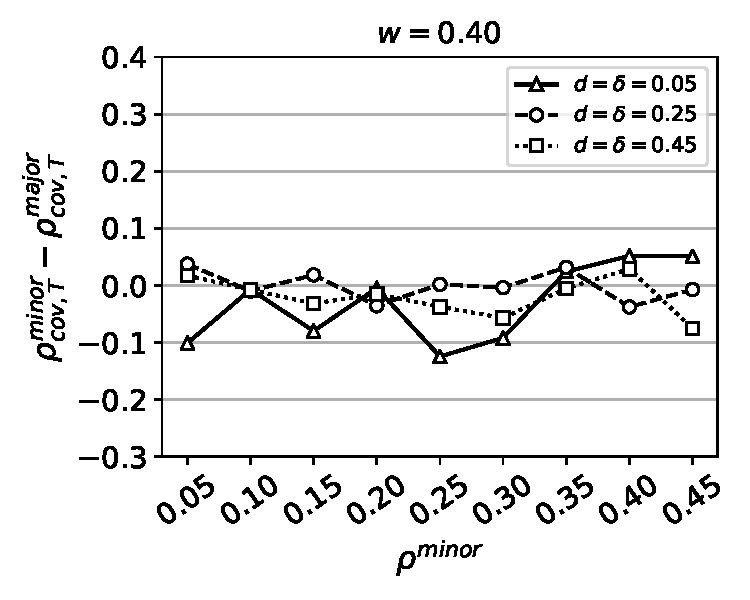
\includegraphics[width=\textwidth]{Figures/full-minority-homophily=0p40.pdf}
  \end{subfigure} \\
  \begin{subfigure}{0.49\textwidth}
    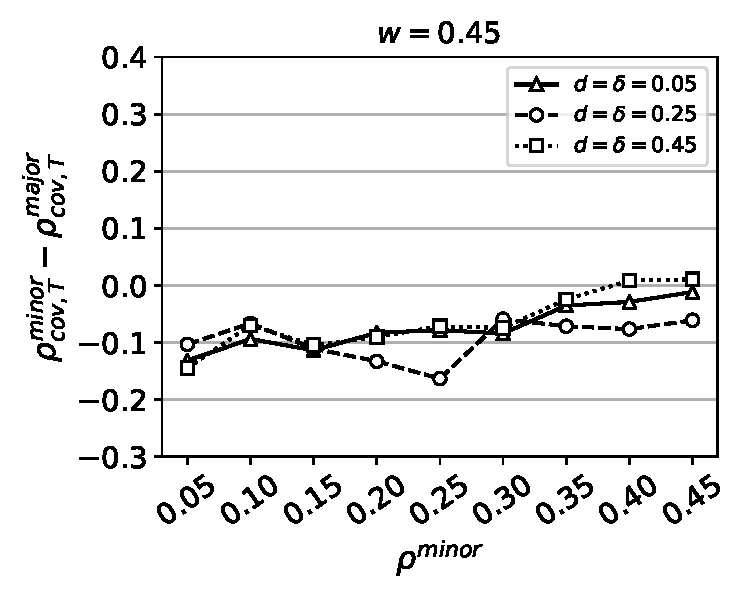
\includegraphics[width=0.7\textwidth]{Figures/full-minority-homophily=0p45.pdf}
  \end{subfigure}
  \begin{subfigure}{0.49\textwidth}
    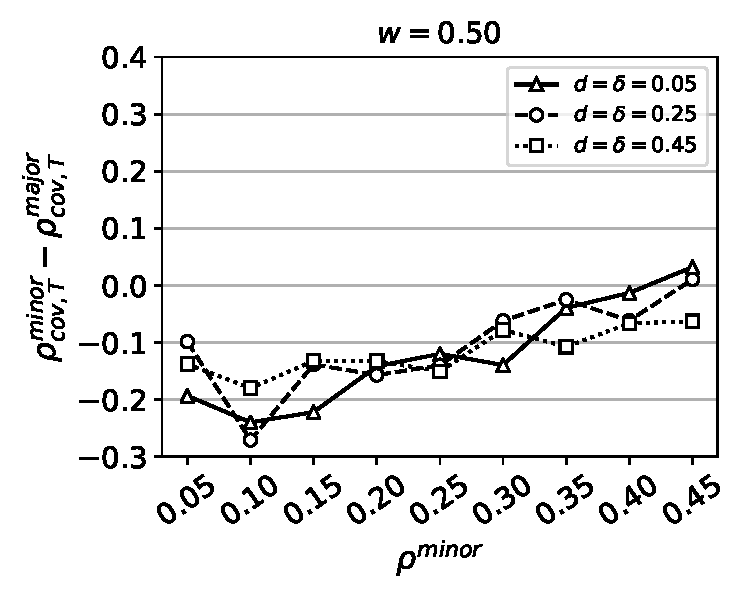
\includegraphics[width=0.7\textwidth]{Figures/full-minority-homophily=0p50.pdf}
  \end{subfigure}
  \caption{}
  \label{fig:}
\end{figure}


\end{appendices}

\end{document}
